%File: formatting-instruction.tex
\documentclass[letterpaper]{article}
\usepackage{latexsym}
\usepackage{url}
\usepackage{float}
\usepackage{amsmath}
\usepackage{algpseudocode}
\usepackage{algorithm}
\usepackage{geometry}
\usepackage{subfig}
\geometry{left=2.0cm,right=2.0cm, top=2.0cm, bottom=2.0cm}
\usepackage{fancyhdr}
\usepackage{longtable}
\usepackage{url}
\usepackage{leftidx}
\usepackage{graphicx,grffile}
\usepackage{epstopdf}
\usepackage{multirow,bigstrut}
\usepackage{booktabs}
\usepackage{amsmath}
\usepackage{subfig}
\usepackage{soul,color}
\renewcommand{\algorithmicrequire}{\textbf{Input:}}
\renewcommand{\algorithmicensure}{\textbf{Output:}}
\newcommand{\algorithmicbreak}{\textbf{break}}
%\usepackage{subcaption}
\usepackage{caption}
\usepackage{aaai}
\usepackage{times}
\usepackage{helvet}
\usepackage{courier}
\frenchspacing
\setlength{\pdfpagewidth}{8.5in}
\setlength{\pdfpageheight}{11in}
\pdfinfo{
/Title (Insert Your Title Here)
/Author (Put All Your Authors Here, Separated by Commas)}
\setcounter{secnumdepth}{0}
 \begin{document}
% The file aaai.sty is the style file for AAAI Press
% proceedings, working notes, and technical reports.
%
\title{Fast Generalized Distillation for Semi-supervised Domain Adaptation}
%\author{AAAI Press\\
%Association for the Advancement of Artificial Intelligence\\
%2275 East Bayshore Road, Suite 160\\
%Palo Alto, California 94303\\
%}
\maketitle
\begin{abstract}
\begin{quote}
Semi-supervised domain adaptation (SDA) can be applied in many real applications. In this paper, we propose our paradigm, called \textit{Generalized Distillation Semi-supervised Domain Adaptation} (GDSDA), that uses the recently proposed framework \textit{Generalized Distillation} (GD) \cite{lopez2015unifying} to solve the SDA problem.
We first theoretically demonstrate the reason why GDSDA can work for SDA problem and show that the imitation parameter can greatly affect the performance of the target model. Then to make GDSDA more practical for real applications, we propose a novel parameter estimation method, called GDSDA-SVM which uses SVM as the base classifier for GDSDA and can effectively estimate the key parameter of GDSDA, i.e. the imitation parameter. Specifically, we use $\ell_2$-loss in GDSDA-SVM and show that we can effectively estimate the imitation parameter by minimizing the Leave-one-out loss of the target model on the training data. Experiment results show that our method can transfer the knowledge between different domains and estimate the imitation parameter effectively for SDA problem.
\end{quote}
\end{abstract}

\section{Introduction}
%An interesting regime for human learners is that it is often sufficient for people to grasp a new category with just a few example and generalize to the novel examples. In machine learning, this scenario is often referred to \textit{learning from sparse label data} (LSLD), such as \textit{one-shot learning scenario} \cite{hoffman2013one}. However, it is difficult for the machine learners to obtain this learning ability as it requires appropriately tuned inductive biases \cite{salakhutdinov2012one}. As a result, in transfer learning, the inductive biases are usually presented as the related source knowledge that can be transferred between tasks. There are many works on investigating transfer learning problem where the labeled data is extremely sparse especially in domain adaptation \cite{hoffman2013one}\cite{pfister2014domain}.
%How to effectively transfer the source knowledge for spares labeled data is still an interesting topic.

Domain adaptation can be used in many real applications, which assumes that the data distribution in the target domain differs from the data distribution in the source domain. Previous methods show that carefully modeling the source data to compensate the domain shift between different domains can significantly improve the performance on the target domain \cite{Donahue_2013_CVPR}. In real applications, it is often very expensive to obtain sufficient labeled examples while there are abundant unlabeled examples in the target domain. 
\textit{Semi-supervised domain adaptation} (SDA) tries to utilize some unlabeled data from the target domain to compensate the domain shift as well as a few labeled data \cite{karl2001long}. Typically, the labeled data are too few to  construct a good classifier alone. How to effectively utilize the unlabeled data is an important issue in SSDA. 

Recently, a framework called \textit{Generalized Distillation} (\textbf{GD}) \cite{lopez2015unifying} was proposed, which allows the knowledge to be transferred between the teacher and student models effectively. GD can be considered as a hybrid framework of two popular paradigms, \textit{Distillation} \cite{hinton2015distilling} and \textit{privileged information} \cite{vapnik2015learning}. In GD, the student learner tries to distill the knowledge of teacher model trained with the privileged information, and mimick the outputs of the teacher model on the training data. Remarkably, GD can be applied in many learning scenarios such as unsupervised, semi-supervised and multitask learning \cite{lopez2015unifying}. Given that GD has such ability in various learning scenarios, people would ask the following two questions: (1) Can GD be applied to solve the SDA problem? (2) Is there any obstacle when we apply GDSDA for real applications?

To answer these two questions, in this paper, we first propose a new paradigm, called \textit{Generalized Distillation Semi-supervised Domain Adaptation} (\textbf{GDSDA}), and illustrate how it can solve the SDA problem. Secondly, we propose a novel algorithm GDSDA-SVM, that makes GDSDA more effective for practical applications. Specifically, to answer the first question, we show that the machine learner trained with our GDSDA framework can effectively exploit the knowledge from the source domain and outperform the source model it learned from when labeled data is sparse.
Different from many other paradigms where the source knowledge is required in both training and testing process, such as \cite{kuzborskij2013stability}, the source knowledge is only required in the training process of GDSDA and the machine learner can work on itself along when testing. More interestingly, we demonstrate that GDSDA can utilize the knowledge from most of the existing classifier.

Then we argue that the imitation parameter of GDSDA controls the amount of knowledge transferred from the source which can greatly affect the performance of the machine learner in real applications (see Section \ref{sec:gdda}).
However, according to previous work \cite{lopez2015unifying,Tzeng_2015_ICCV}, the imitation parameter can only be determined by either brute force search or background knowledge. It is ideal to find a method that can determine the imitation parameter automatically, especially when there are more than one imitation parameter to be determined.

Therefore, we propose a novel imitation parameter estimation method for GDSDA, called GDSDA-SVM that uses SVM as the base learner and can determine the imitation parameter automatically. In particular, inspired by \cite{cawley2006leave}, we use $\ell_2-$loss for GDSDA-SVM and show that the Leave-one-out cross validation (LOOCV) loss can be calculated in a closed form. By minimizing the LOOCV loss on the target training data, we can find the optimal imitation parameter for the target model. In our experiments, we show that GDSDA-SVM can effectively find the optimal imitation parameter and achieve competitive performance compared to methods using brutal force search. In addition, the main contributions of this paper include: (1) We propose the framework GDSDA for domain adaptation and show that GDSDA can be used in many domain adaptation problems. (2) We propose the GDSDA-SVM that can effectively find the optimal imitation parameter for GDSDA.

The rest of this paper is organized as follow: In Section \ref{sec:work}, we describe the related work on privileged information and distillation in domain adaptation. Section \ref{sec:gdda} we propose our framework of GDSDA and provide some statistic analysis. Based on that, we propose our GDSDA-SVM in Section \ref{sec:svm}. Experimental results are shown in Section \ref{sec:exp}. Some discussion and conclusion are provided in Section \ref{sec:con}.

%The problem of machines-teaching-machines has become an interesting topic in machine learning area. This problem focuses on how to let the student machines learn from their teacher machines effectively, in addition to training data.

Similar to our human teaching scenario, a typical paradigm for this problem is using the intelligent teacher to provide privileged information for the student model in the learning process while the student model has no access to the privileged information at the test time \cite{vapnik2009new}\cite{vapnik2015learning}. On the other hand, using the soft output from an ensemble of models to train a single model, known as \textit{Distillation} demonstrates its ability to transfer the knowledge between models in many real world applications  \cite{Gupta_2016_CVPR}\cite{hinton2015distilling}\cite{luo2016face}\cite{Tzeng_2015_ICCV}\cite{urban2016deep}. 

A recent framework unifies this two approaches together and train the student model by distilling the knowledge from a teacher model trained with privileged information, which is referred to as \textit{Generalized Distillation} \cite{lopez2015unifying}. This framework can be applied to many learning tasks, such as semi-supervised learning and multi-task learning. It is reasonable to apply Generalized Distillation to \textit{Domain Adaptation}, called \textit{Generalized Distillation Domain Adaptation} (\textbf{GDDA}), where we treat the source model as the teacher model to provide the soft label for the examples in the target domain in the training process to train the model for the target domain.  
There are several advantages for GDDA,
such as compatible with various of classifiers and scenarios, highly effective in small data regimes (For more details, see Section \ref{sec:gdda}).

In Generalized Distillation, the imitation parameter controls the importance of the teacher model. Accordingly, in GDDA, the imitation parameter controls the amount of the knowledge transferred from the source model. We show that the imitation parameter determines the quality of the transfer process, i.e. the performance of the target model (see Section \ref{sec:gdda}). In previous work, this imitation parameter can only be determined  by either brute force search or background knowledge \cite{lopez2015unifying}\cite{Tzeng_2015_ICCV}. It is not clear how to determine the value of imitation parameter effectively, which become more crucial especially for the multi-source scenario in domain adaptation, where there could be multiple imitation parameters to be determined.

\begin{figure}
\centering
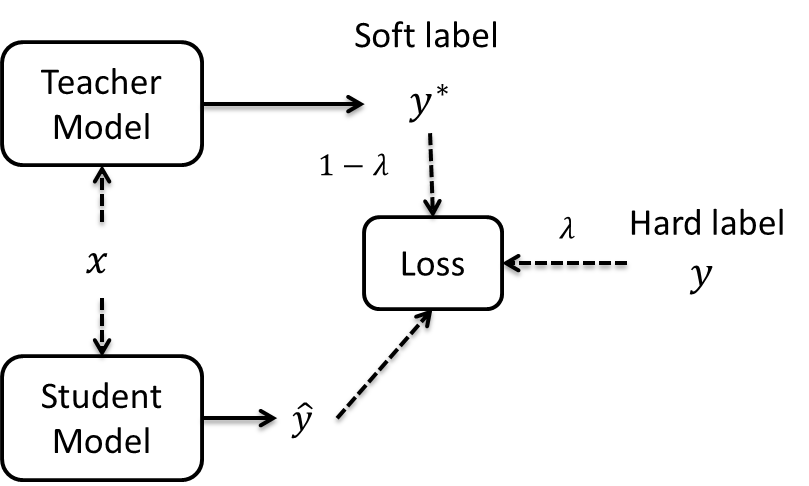
\includegraphics[scale=.8]{figure/GDDA.png}
\caption{Illustration of GDDA training process.}
\end{figure}
In this paper, we propose a novel method for GDDA, called GDDA-SVM that can determine the imitation parameter automatically. In particular, inspired by \cite{cawley2006leave}, we use $\ell_2-$loss for GDDA-SVM and show that the Leave-one-out cross validation (LOOCV) loss can be calculated in a closed form. By minimizing the LOOCV loss on the target training data, we can find the optimal imitation parameter for the target model. In our experiments, we show that GDDA-SVM can effectively find the optimal imitation parameter and achieve better performance compared to methods using brutal force search. The main contributions of this paper include: (1) We propose the framework GDDA for domain adaptation. (2) We propose a method GDDA-SVM for imitation parameter estimation.

The rest of this paper is organized as follow: In Section \ref{sec:work}, we describe the related work on privileged information and distillation in domain adaptation. Section \ref{sec:gdda} we propose our framework of GDDA and provide some statistic analysis. Based on that, we propose our GDDA-SVM in Section \ref{sec:svm}. Experimental results are shown in Section \ref{sec:exp}. Some discussion and conclusion are provided in Section \ref{sec:con}.

%For our human, a good student can learn a new concept very fast under the supervision of the teacher with just a few examples and make meaningful generalizations to novel instances. 

%\section{Background}
%\textit{Distillation for domain adaptation} \cite{hinton2015distilling} and \textit{privileged information} \cite{vapnik2015learning} are two techniques that enable machines to learn from other machines. Both methods address the problem how to build a student model that can learn from the advanced teacher models. Recently, Lopez \textit{et al.} \cite{lopez2015unifying} proposed a framework called \textit{generalized distillation} that unifies both techniques and show that it can be applied in many scenarios.
\subsection{Privileged information}
In the original work of the privileged information \cite{vapnik2015learning}, the data can be represented as a collection of the triples:
\[\{\left(x_1,x_1^*,y_1\right),\left(x_2,x_2^*,y_2\right) \dots \left(x_n,x_n^*,y_n\right)\}\]
where each $(x_i,y_i)$ is a feature-label pair, and the novel element $x_i$ is additional information about the example $(x_i,y_i)$ provided by an intelligent teacher, such as to support the learning process. However, in the testing procedure, the learning machine is not able to obtain the privileged information from the teacher. Vapnik's learning using privileged information is one example of what we call machines-teaching machines: the paradigm where machines learn from other machines, in addition to training data. 
\subsection{Distillation}
Distillation uses a simple (student) machine learns a complex task by imitating the solution of a flexible (teacher) machine. For a $c$-class scenario, distillation works as follow: consider the data
\[\{x_i,y_i\}_{i=1}^n, \qquad x\in R^d, y\in \Delta^c\]
where $\Delta^c$ is a $c$-dimensional probability vector. In traditional learning, we try to learn a function $f_t$ that:
\begin{equation}\label{eq:normal}
f_t=\underset{f_t \in \mathcal{F}_t}{\arg \min}\frac{1}{n}\sum_{i=1}^{n}\ell\left(y_i,\sigma(f_t(x_i))\right)+\Omega(||f_t||)
\end{equation}
here $\sigma$ is the softmax operation:
\[\sigma(z)_k=\frac{e^{z_k}}{\sum_{j=1}^{c}e^{z_j}}\]
and $\ell$ is the cross-entropy loss function:
\[\ell(y,\hat{y})=-\sum_{i=1}^{c}y_i\log\hat{y}_i\]
In distillation, we try to learn the student machine $f_s$ to imitate the teacher machine $f_t$. During the learning process, $f_s$ can receive the soft label $s_i$ from the teacher machine $f_t$ for each training example $x_i$.
\begin{equation}\label{eq:softmax_T}
s_i=\sigma(f_t(x_i)/T)
\end{equation}
where $T$ is the temperature for distillation. It is worthy to note that in distillation, $f_t$ can either be a single large complex neural network or an ensemble of some complex classifiers. We can see that the soft label $s_i$, which reveals the class dependency, is more informative than the class label $y_i$.

The student machine can be learned by:
\begin{equation}\label{eq:distill}
f_s=\underset{f_s \in \mathcal{F}_s}{\arg \min}\frac{1}{n}\sum_{i=1}^{n}\left[\lambda\ell\left(y_i,\sigma(f_s(x_i))\right)+(1-\lambda)\ell\left(s_i,\sigma(f_s(x_i))\right)\right]
\end{equation}
here, $\mathcal{F}_s$ is a simpler function class than $\mathcal{F}_t$ and $\lambda$ is the imitation parameter to balance the importance between the hard label $y_i$ and the soft label $s_i$. The temperature $T>0$ controls how do we want to smooth the probability from the teacher $f_t$. Higher temperature leads to softer label.

\subsection{Generalized distillation}
Generalized distillation (GD) tries to unify the two frameworks together while using the soft label as the privileged information. The process of generalized distillation is as follows:

\begin{enumerate}
\item Learn teacher ${f}_t$ using the input-output pairs $\{x^*_i,y_i\}_{i=1}^n$ and Eq. \ref{eq:normal}.
\item Compute teacher soft labels $s_i$, using the temperature parameter $T > 0$.
\item Learn the student ${f}_s$ using the pair $\{\left(x_i,y_i\right),\left(x_i,s_i\right)\}_{i=1}^n$ and imitation parameter $\lambda$.
\end{enumerate}

\section{Related Work}\label{sec:work}
As we use GD to solve SDA problem, we will introduce the related work on both areas.

In SDA, many works have been proposed to utilize the unlabeled data. Yao {et al.} \cite{yao2015semi} proposed a framework, named Semi-supervised Domain Adaptation with Subspace Learning (SDASL) to correct data distribution mismatch and leverages unlabeled data. Donahue {et al.}\cite{Donahue_2013_CVPR} proposed a framework for adapting classifiers by "borrowing" the source data to the target domain using a combination of available labeled and unlabeled examples. Daume {et al.} \cite{daume2010frustratingly} proposed a method by augmenting the feature space to compensate the domain shift. Duan {et al.} \cite{duan2012visual} proposed a method using the unlabeled data to measure the mismatch between the domains based on the maximum mean discrepancy.

There are also many works related to GD in computer vision community. Sharmanska et al. \cite{Sharmanska_2013_ICCV} proposed a Rank Transfer method that uses attributes, annotator
rationales, object bounding boxes, and textual descriptions as the privileged information for object recognition. Motiian et al. \cite{Motiian_2016_CVPR} proposed {the information bottleneck method with privileged information (IBPI)} that leverage the auxiliary information such as like supplemental visual features, bounding box annotations and 3D skeleton tracking data to improve visual recognition performance. Tzeng et al. \cite{Tzeng_2015_ICCV} proposed a CNN architecture for domain adaptation to leverage the knowledge from limited or no labeled data using the soft label. Urban et al. \cite{urban2016deep} use a small shallow net to mimick the output of a large deep net while using layer-wised distillation with $\ell_2$ loss of the outputs of student and teacher net. Similarly, Luo et al. \cite{luo2016face} use $\ell_2$ loss to train a compressed student model from the teacher model for face recognition. Gupta et al. \cite{Gupta_2016_CVPR} use supervision transfer to distill the knowledge from a trained CNN with unlabeled data or just a few labeled data.

\section{Generalized Distillation for Semi-supervised Domain Adaptation}\label{sec:gdda}
As we mentioned, GDDA is a paradigm using generalized distillation for domain adaptation. In this section, we first give a brief review of generalized distillation. Then we show the process of GDDA and demonstrate the reason why GDDA can work with the SSDA problem. Finally, we show that to achieve an optimal model, we should carefully set the value of imitation parameter to minimize the training error. 
\begin{figure}
\centering
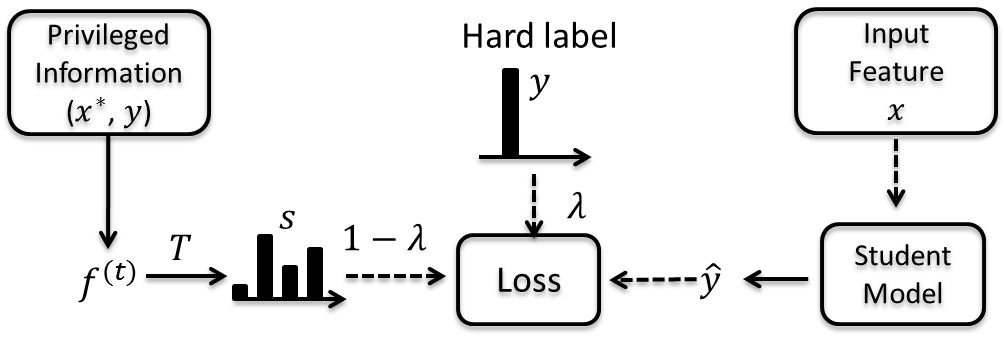
\includegraphics[scale=.4]{figure/GD.png}
\caption{Illustration of Generalized Distillation training process.}
\end{figure}
\subsection{An overview of generalized distillation and GDDA}
\textit{Distillation} \cite{hinton2015distilling} and \textit{Learning Using Privileged Information} (LUPI) \cite{vapnik2015learning} are two paradigms that enable machines to learn from other machines. Both methods address the problem how to build a student model that can learn from the advanced teacher models. Recently, Lopez {et al.} \cite{lopez2015unifying} proposed a framework called \textit{generalized distillation} that unifies both techniques and show that it can be applied in many scenarios.

In GD, the training data can be represented as a collection of the triples:
\[\{\left(x_1,x_1^*,y_1\right),\left(x_2,x_2^*,y_2\right) \dots \left(x_n,x_n^*,y_n\right)\}\]
where $x^*$ is the privileged information associate to the label $y$ which is not accessible in the test process. Therefore, the goal of GD is to train a model, called student model with the guidance of the the privileged information.

The process of generalized distillation is as follows: in step 1, a teacher model ${f}^{(t)}$ is trained using the input-output pairs $\{x^*_i,y_i\}_{i=1}^n$. In step 2, use ${f}^{(t)}$ to generate the soft label $s_i$ for each training example $x_i$ using with the softmax function $\sigma$:
\begin{equation}\label{eq:softmax_T}
s_i=\sigma(f^{(t)}(x_i)/T)
\end{equation}
where $T$ is a parameter called temperature to control the smoothness of the soft label. In step 3, learn the student ${f}^{(s)}$ using the pair $\{\left(x_i,y_i\right),\left(x_i,s_i\right)\}_{i=1}^n$ using:
\begin{equation}\label{eq:distill}
\begin{aligned}
f^{(s)}=&\underset{f^{(s)} \in \mathcal{F}^{(s)}}{\arg \min}\frac{1}{n}\sum_{i=1}^{n}[\lambda\ell\left(y_i,\sigma(f^{(s)}(x_i))\right)\\
&+(1-\lambda)\ell\left(s_i,\sigma(f^{(s)}(x_i))\right)]\\
\end{aligned}
\end{equation}
Here, $\lambda$ is the imitation parameter to balance the importance between the hard label $y_i$ and the soft label $s_i$.


GD can be used in many scenarios such as multi-task learning, semi-supervised learning, and reinforcement learning. As generalized distillation only required for the training inputs $\{x_i,y_i\}_{i=1}^n$ and the output $s$ from the teacher function $f_t$, it can be naturally applied in domain adaptation, called \textit{Generalized Distillation Semi-supervised Domain Adaptation} (\textbf{GDSDA}), where the source model can be used as the teacher to output the soft labels and the student model is the target model. To be consistent with other works in domain adaptation, we use source model and target model to denote the teacher model and the student model in the rest of our paper respectively.

An important issue the extend GD to SDA is that, in Eq. \eqref{eq:distill}, each example is assigned a hard label (ground truth) and a soft label. However, in SDA, we are not able to obtain the hard label for unlabeled data. Here similar to GD \cite{lopez2015unifying}, we use the "fake label" strategy to the unlabeled data: for the labeled examples, we use \textit{one-hot} strategy to encode their labels while use gray code (all 0s) to the unlabeled examples as their label. Thus, each example in the target domain has its own label now. It is reasonable to argue that the "fake label" strategy would introduce extra noise and degrade the performance. However, we will show in our experiment that when the labeled examples are rare, we can still achieve improved performance by setting the proper value to the imitation parameter (See the single source experiment in Section \ref{sec:exp}).

Suppose we have $M-1$ source domains denoted as $D_s^{(j)}=\{X^{(j)},Y^{(j)}\}_{j=1}^{M-1}$ and the target domain $D_t=\{\{X,Y\}$ encoded with the "fake label" strategy. Similar to GD, the process of GDSDA is as follow:
\begin{enumerate}
    \item Train the source models $f^*_j$ for each of the $M-1$ domain with $\{X^{(j)},Y^{(j)}\}$.
    \item For each of the training example $x_i$ in the target domain, computer the corresponding soft label $y^*_{ij}$ with each of the source model $f^*_j$ and some temperature $T>0$.
    \item Learn the target model $f_t$ using the $(M+1)$-tuple $\{x_i,y_i,y^*_{i1},\dots,y^*_{M-1}\}_{i=1}^L$ with some imitation parameters $\{\lambda_i\}^M_{i=1}$ using \eqref{eq:GDDA_abs}:
\end{enumerate} 
\begin{equation}\label{eq:GDDA_abs}
\begin{aligned}
f_t(\lambda)=&\underset{f_t \in \mathcal{F}}{\arg \min}\frac{1}{L}\sum_{i=1}^{L}[\lambda_1\ell\left(y_i,f_t(x_i)\right)+\\&\sum_{j=1}^{M-1}\lambda_{j+1}\ell\left(y^*_j,f_t(x_i)\right)]\qquad
 \text{s.t.} \qquad \sum_i\lambda_i=1
\end{aligned}
\end{equation}
Compared to other works of SDA which require to utilize each example of the source domain, by either re-weighting \cite{Donahue_2013_CVPR,duan2012visual} or augmentation \cite{daume2010frustratingly}, GDSDA only requires the trained model from the source domain to generate the soft label. Considering the fact that it is more convenient to manipulate the source model than each of the examples in the source domain, GDSDA can be more effective than those previous method. For example, if we want to use ImageNet \cite{imagenet_cvpr09} as the source domain, it is almost impossible to access each of the millions of the examples while there are many well trained models publicly available online to be leveraged. Also, GDSDA is able to handle the multi-class scenario while some previous work, such as SHFA\cite{duan2012learning} can only solve the problem of binary class in SSDA. Moreover,it is clear that GDSDA is compatible with any type of source model that can output the soft label.

\subsection{Statistic analysis of GDSDA}
In this part, we provide statistic analysis for the scenarios where GDSDA would work. Before we provide the analysis, there are two basic assumptions for GDSDA to work well in domain adaptation: the \textit{assumption of distillation and the assumption of  transfer}.

\textbf{Assumption of Distillation:} The capacity (i.e. VC dimension) of target model $f_t$ is smaller than the capacity of source model $f^*$. This assumption is inherited from distillation.
\textbf{Assumption of Transfer:} The source model $f^*$ should work better than a target model $f'_t$ trained only with the hard labels. For example, when we only have a single labeled example for each class in the target training set, it is reasonable to assume that some source models trained from other domain could perform better than any model trained only with the target training data on the target task.

Let $\hat{R}(f)$ be the training error of the model $f$ with finite VC dimension $h$ on a training data with size $L$. According to ERM principle, the generalization error bound $R(f)$ of the model is:
\begin{equation}
R(f) \leq \hat{R}(f)+O\left(\sqrt{\frac{h}{L}}\right)
\end{equation}
As long as the target model can achieve similar training error on the target training data to the training error of the source model, i.e. $\hat{R}(f_t) \approx \hat{R}(f^*)$, it could have better generalization error than the source model, i.e. $R(f_t)\le R(f^*)$ \cite{hinton2015distilling}. 
%Previous work \cite{hinton2015distilling} suggests that if the target model can simulate the outputs of the source model, i.e. the soft label, well enough on the training data, the target model could outperform the source model on this task. 
It is worthy to notice that in this process, we don't require any labeled examples from the training set. This means GDSDA can effectively utilize the unlabeled data in SDA problem.

Arguably, the source model is biased on the target task due to the domain shift. More interestingly, as it is suggested in \cite{hinton2015distilling}, we can use some labeled data from the target domain to adjust the bias and achieve a better performance on the target task with Eq. \eqref{eq:distill}. This indicates that the target model trained with GDSDA can be further improved with the help of a few labeled data. Here, we use the imitation parameter $\lambda$ to control the importance of the soft label from the source model and the true label, i.e. the similarity between the source and target tasks. In addition, GDSDA can effectively utilize the unlabeled data to transfer the knowledge from source domain while using a few labeled data to compensate the domain shift (see the experiment results in Section \ref{sec:exp}).

\subsection{Key parameter: the imitation parameter}\label{sec:key}
From above we can see that GDSDA can effectively transfer the knowledge between source and target tasks. In this part, we theoretically demonstrate that the imitation parameter can greatly affect the performance of the target model.

In GDSDA, we have to decide the values of 2 parameters, the temperature $T$ and imitation parameter $\lambda$. The temperature $T$ control the smoothness of the soft label and the imitation parameter $\lambda$ controls how similar the target model is to the source model. Many previous works have addressed the importance of the similarity control when transferring the knowledge between different domains \cite{duan2012learning,duan2012visual}. Without carefully controlling the amount of the knowledge transferred from the source domain, it is easy for the target model to get degraded performance or even suffer from negative transfer \cite{pan2010survey}.
Here we show that the value of imitation parameter can greatly affect the performance of the target model. Specifically, we show that we should choose the imitation parameter that minimizes the empirical risk on the training data for distillation.

Let $f(x,\lambda)$ be a function with a finite VC dimension $h$ that minimizes the number of errors on the training data $\{x_i,y_i\}_{i=1}^L$. Let $v(\lambda)$ be the training error. Then according to the VC theory \cite{vapnik1999overview}, for an arbitrary loss function $\mathcal{L}(\cdot)$ we have the following bound:
\begin{equation}\label{eq:lambda_constraint}
P\left(\mathcal{L}\left(y,f(x,\lambda)\right)\geq 0\right) < v(\lambda)+O\left(\sqrt{\frac{h}{L}}\right)
\end{equation}
In other word, the optimal imitation parameter should be the one that can minimize the training error.  

In the previous work, the imitation parameter can only be determined by either brute force search \cite{lopez2015unifying} or background knowledge \cite{Tzeng_2015_ICCV} which greatly reduces its effectiveness. In domain adaptation, it is common that there could be multiple source models to be exploited. It is ideal to find a method that can determine the imitation parameter automatically.


\section{GDSDA-SVM}\label{sec:svm}
%As we mentioned above, to achieve the best performance of the target model, the imitation parameter should be set to minimize the training error. 
As we mentioned, it is important to find a method that can determine the imitation parameter effectively. In this section, we propose our method GDSDA-SVM that uses SVM as the base classifier and can effectively estimate the imitation parameter by minimizing the training error on the target domain.
\subsection{Distillation with multiple sources}
%As we discussed above, we should find a method that can estimate the optimal imitation parameter effectively for real applications. 
%To solve this problem, we propose a novel method that uses SVM as the base classifier and can determine the imitation parameter $\lambda$ autonomously, called GDSDA-SVM. 
As it is suggested in \cite{vapnik2015learning}, the optimal imitation parameter should be the one that can minimize the training error on the target domain. Based on that, we propose our method GDSDA-SVM that can estimate the imitation parameter effectively.

In our GDSDA-SVM, instead of using hinge loss, we use Mean Squared Error (MSE) as our loss function for the following two reasons: (1) Several recently works \cite{ba2014deep,luo2016face,romero2014fitnets,urban2016deep} show that MSE is also an efficient measurement for the target model to mimick the behavior of the source model. (2) MSE can provide a closed form cross-validation error estimation. Thus we can effectively estimate the imitation parameter. 

\begin{figure}\label{fig:GDSDA}
\centering
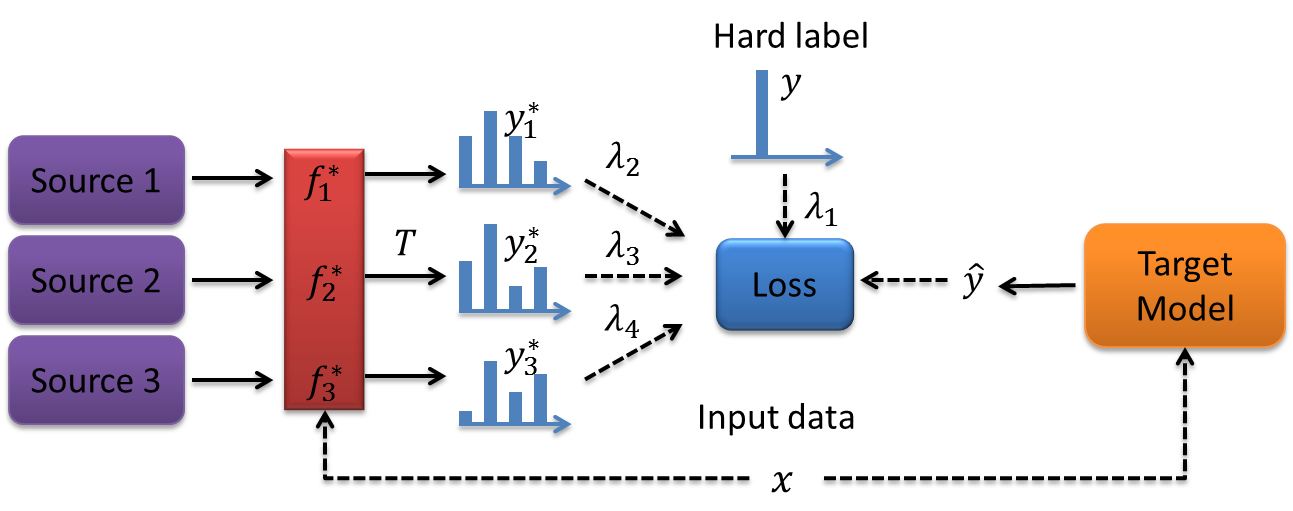
\includegraphics[scale=.3]{figure/multi-GDDA.png}
\caption{Illustration of GDSDA training process.}
\end{figure}

Suppose we have $L$ examples $\{\textbf{x}_j,\textbf{y}_j\}_{j=1}^L$ from and $N$ classes in the target domain where $X\in R^{L\times d}, Y\in R^{L\times N}$. Meanwhile, there are $M-1$ the source (teacher) models providing the soft labels $Y^*=\{\textbf{y}^*_{ij}|j=1,...,L;i=1,...,M-1\}$ for each of the $L$ examples.
For simplicity, we combine the hard label $Y$ and soft label $Y^*$ and use new label matrix: $S \in R^{M\times L \times N}$ to denote them. To solve this $N$-class classification problem, we adopt the One-vs-All strategy to build $N$ binary SVMs.
To obtain the $n$th binary SVM, we have to solve the following optimization problem: 
\begin{equation}\label{eq:multi-distill}
\begin{aligned}
\min \qquad & \frac{1}{2}{|| \textbf{w}_n ||^2} + C\sum_{i,j} \lambda_i{e_{ijn}^2} \\
s.t.\qquad& e_{ijn} = s_{ijn} - \textbf{w}_n\textbf{x}_j\\
& \sum_i\lambda_i=1; \lambda_i \in [0,1]; i\in M;  j\in L\\
\end{aligned}  
\end{equation}
To solve this optimization problem, we use KKT theorem \cite{cristianini2000introduction} and add the dual sets of variables to the Lagrangian of the optimization problem:
\begin{equation}
\begin{aligned}
\mathcal{L}=&\frac{1}{2}{|| \textbf{w}_n ||^2} + C\sum_{i,j} \lambda_i{e_{ijn}^2}+\sum_{i,j}\alpha^{(n)}_{ij}\left(s_{ij} - \textbf{w}_n\textbf{x}_j-e_{ij}\right)\\&+\beta^{(n)}\left(\sum_i\lambda_i-1\right)
\end{aligned}
\end{equation}
To find the saddle point, 
\begin{equation}
\begin{aligned}
\frac{{\partial L}}{{\partial \textbf{w}_n}}& = \textbf{w}_n - \sum_{j}\alpha^{(n)}_{ij} {\textbf{x}_j}=0 \rightarrow \textbf{w}_n = \sum_{j}\alpha^{(n)}_{ij} {\textbf{x}_j}\\
\frac{{\partial L}}{{\partial {e_{ijn}}}} & = 2C\lambda_i {e_{ijn}} - {\alpha^{(n)} _{ij}}=0 \rightarrow \alpha^{(n)}_{ij} = 2C\lambda_i {e_{ijn}}\\
\end{aligned}
\end{equation}
For each example $\textbf{x}_j$ and its constraint of label $s_{ijn}$, we have $e_{ijn}  + \textbf{w}_n\textbf{x}_j= s_{ijn}$. Replacing $\textbf{w}_n$ and $e_{ijn}$,  we have:  
\begin{equation}
\begin{aligned}
%x_j\sum_{k}\alpha^{(n)}_{ik}x_k+\frac{\alpha^{(n)}_{ij}}{2C\lambda_i}&=s_{ijn}\\
\lambda_i\textbf{x}_j\sum_{k}\alpha^{(n)}_{ik}\textbf{x}_k+\frac{\alpha^{(n)}_{ij}}{2C}&=\lambda_is_{ijn}
%x_j\sum_{k}\alpha^{(n)}_{ik}x_k+\sum_j\frac{\alpha^{(n)}_{ij}}{2C}&=\sum_j\lambda_js_{ijn}
\end{aligned}
\end{equation}
Summing over each constraint of example $x_j$, we have:
\begin{equation}
\underbrace{\sum_i\lambda_i}_{=1} \textbf{x}_j\sum_{k}\alpha^{(n)}_{ik}\textbf{x}_k+\sum_i\frac{\alpha^{(n)}_{ij}}{2C}=\sum_i\lambda_is_{ijn}
\end{equation}
%Here we use $K$ to denote the kernel matrix $K=\{x_ix_j|i,j\in 1\dots L\}$.
Let %$M=[K+\frac{\mathbf{I}}{2C}]$ and 
$\eta_{jn}=\sum_i\alpha^{(n)}_{ij}$, we have:
\begin{equation}
\begin{aligned}
\sum_j\eta_{jn}\textbf{x}_jx_i+\frac{\eta_{in}}{2C}&=\sum_i\lambda_is_{ijn}\\
%M\eta_n&=S_n\begin{bmatrix}
%\lambda_1\\\vdots\\\lambda_m
%\end{bmatrix}
\end{aligned}
\end{equation}

This implies that solving the optimization problem \eqref{eq:multi-distill} is equivalent to solve a standard LS-SVM \cite{suykens1999least} whose the target is the weighted sum of each label $\sum_i\lambda_is_{ijn}$.

Here we use $\Omega$ to denote the matrix $\Omega=[K+\frac{\mathbf{I}}{2C}]$ where $K$ is the kernel matrix $K=\{\textbf{x}_i\textbf{x}_j|i,j\in 1\dots L\}$. To simplify our notation, let ${\eta}'_{n}=M^{-1}S_n$ where $S_n$ is the matrix $S_n=\{s_{ijn}|i\in M;j\in L\}$ and $\Omega^{-1}$ is the inverse of matrix $\Omega$. 

Let $\eta_{jn}=\sum_i\lambda_i{\eta}'_{ijn}$.
The Leave-one-out estimation of the example $\textbf{x}_j$ for the $n$th binary SVM can be written as \cite{cawley2006leave}:
\[\sum_i\lambda_is_{ijn}-\hat{y}_{jn} =\frac{{\eta}_{jn}}{\Omega_{jj}^{-1}} =\frac{\sum_i\lambda_i{\eta}'_{ijn}}{\Omega_{jj}^{-1}}\]
\begin{equation}\label{eq:yhat}
\hat{y}_{jn} = \sum_i\lambda_i\left(s_{ijn}-\frac{{\eta}'_{ijn}}{\Omega_{jj}^{-1}}\right)
\end{equation}
where $\Omega^{-1}_{jj}$ is the $j$th diagonal element of $\Omega^{-1}$. Now for any given $\lambda$, we have found an efficient way to estimate the LOO of each binary target model for example $\textbf{x}_j$. In the following part, we will introduce how to find the optimal $\lambda_i$ for each of the source models. 
\subsection{Cross-entropy loss for imitation parameter estimation}
From the previous part, we have already found a effective way to estimate the output of the SVM. The optimal imitation parameters, can be found by solving the following optimization problem:
\begin{equation}\label{eq:loo_loss}
\begin{aligned}
\min \quad& L_c\left(\lambda\right)=\frac{1}{2}\sum_i^M||\lambda_i||^2+\frac{1}{L}\sum_{j,n}\ell\left(y_{in},\hat{y}_{jn}\left(\lambda\right)\right)\\
s.t. \quad& \sum\lambda_i=1
\end{aligned}
\end{equation}
Here we use the $\ell$-2 regularization term to control the complexity of $\lambda$s so that the target model can achieve better generalization performance. For the loss function $\ell(\cdot,\cdot)$, We use the cross-entropy loss function.
\begin{equation}\label{eq:ce}
\begin{aligned}
\ell\left(y_{in},\hat{y}_{jn}\left(\lambda\right)\right)=&y_{in}\log(P_{jn})\\
P_{jn} =& \frac{e^{\hat{y}_{jn}}}{\sum_{h} e^{\hat{y}_{jh}}}
\end{aligned}
\end{equation}
Cross-entropy pays less attention to a single incorrect prediction which reduces the affect of the outliers in the training data. Moreover, cross-entropy works better for the unlabeled data with our "fake label" strategy. As we mentioned in our "fake label" strategy, we use one-hot strategy to encode the hard labels of the labeled examples while encoding the unlabeled examples with gray code. When we use cross-entropy, it can automatically ignore penalties of the unlabeled examples and reduce the noise introduced by our "fake label" strategy. 
Let:
\begin{equation}\label{eq:mu}
\begin{aligned}
\mu_{ijn}=s_{ijn}-\frac{{\eta}'_{ijn}}{\Omega_{jj}^{-1}} \qquad
\end{aligned}
\end{equation}
The derivative can be written as:
\begin{equation}\label{eq:p}
\begin{aligned}
\frac{\partial \ell(\lambda)}{\partial \lambda_i}&=\sum_n\mu_{ijn}\left(P_{jn}-{y}_{jn}\right)
\end{aligned}
\end{equation}
\begin{algorithm}[t]
	\caption{GDSDA-SVM}\label{alg:svm}
	\begin{algorithmic}
		\Require Input examples $X=\{\textbf{x}_1,...,\textbf{x}_L\}$, number of classes $N$, number of sources $M$, 3D label matrix, $S=[Y_1,Y_2,...,Y_{M}]$ with size $L\times M \times N$, temperature $T$ %optimization iteration $iter$
		\Ensure Target model $f_t = Wx$
		\State Compute $\Omega=[K+\frac{\mathbf{I}}{2C}]$
		\State Compute imitation parameter $\lambda$ with Algorithm \ref{alg:lambda}
		\State Compute new label $Y_{new}=\sum_i\lambda_iY_i$
		\State Compute $\eta = \Omega^{-1}Y_{new}$
		\State Compute $w_n = \sum_j \eta_{jn}x_j$
	\end{algorithmic}	
\end{algorithm}
\begin{algorithm}[t]
	\caption{$\lambda$ Optimization}\label{alg:lambda}
\begin{algorithmic}
	\Require Input examples $X$, number of classes $N$, size of sources $M$, 3D label matrix $S$, temperature $T$, optimization iteration $iter$, Kernel matrix $\Omega$
    \Ensure Imitation parameter $\lambda$
    \State Initialize $\lambda = \frac{1}{M}$, 
    
    \State Let $S_n$ be the label matrix of $S$ for class $n$
    \For{Each label $S_n$} 
    \State Compute $\eta'_n=\Omega^{-1}S_n$ 
    \EndFor
    \State Compute $\mu$ using \eqref{eq:mu}
    \For {$it \in \{1,...,iter\}$ }
	    \State Compute $\hat{y}_{jn}$ and $P_{jn}$ with \eqref{eq:yhat}  and \eqref{eq:ce}
	    \State $\Delta_{\lambda} \leftarrow 0$
	    \For {each $\textbf{x}_j$ in $X$}
		    \State $\Delta_{\lambda} = \Delta_{\lambda}+\sum_n\mu_{ijn}\left(P_{jn}-{y}_{jn}\right)$
	    \EndFor
	    \State $\Delta_{\lambda} =\Delta_{\lambda}/L$, $\lambda = \lambda - \frac{1}{it}(\Delta_{\lambda}+\lambda)$
	    \State $\lambda = \lambda / \sum\lambda_i$
%	    \State 
    \EndFor
\end{algorithmic}	
\end{algorithm}
To summarize, we describe GDSDA-SVM in Algorithm \ref{alg:svm}. As the optimization problem \eqref{eq:loo_loss} is strongly convex, it is easy to prove that Algorithm \ref{alg:lambda} can converge to the optimal $\lambda$ with the rate of $O(\log(t)/t)$ where $t$ is the optimization iteration (The proof is shown in Supplemental Material). 






\section{Experiments}\label{sec:exp}
We verify our algorithm GDDA-SVM on the benchmark dataset Office. Moreover, we provide two different settings: single source and multi-source scenarios for GDDA-SVM.
\subsection{Dataset}
There are 3 subsets in offices datasets, Webcam (795 examples), Amazon (2817 examples) and DSLR (498 examples), sharing 31 classes. In our experiments, we use DSLR and Webcam as the source domain and Amazon as the target domain.
We use the features extracted from Alexnet \cite{KrizhevskyNIPS12} FC7 as the input features for both source and target domain. The source model is trained with multi-layer perception (MLP) on the whole source dataset. 

\subsection{Single Source for Office datasets}
As we mentioned, there are significantly fewer labeled examples than unlabeled ones in real SSDA applications. In this experiment, we compare our algorithm with the baselines in this situation where there is just one source model that generates the soft label. Specifically, we perform two groups of experiment using Amazon dataset as the target domain and DSLR and Webcam datasets as the source domain respectively. In each group of experiment, we show 3 results with different settings. We set the size of the labeled example to be 1 per class, and the size of the unlabeled example to be 10, 15 and 20 per class respectively.

To show the effectiveness of GDDA-SVM, we also use brute force to search the imitation parameter $\lambda$ in the range $[0,0.1,...,1]$ for comparison with different temperature $T$. We also show the performance of the source model on the target task, denoted as "Source" and the performance of a target model trained with only labeled examples in the target domain denoted as "No transfer". To avoid the randomness, we perform each experiment 10 times and report the average results. In GDDA-SVM, we use temperature $T=20$. The experimental results are shown in figure \ref{fig:single1}. The imitation parameter of the figures denotes the imitation parameter $\lambda$ for the hard label and the corresponding imitation parameter for the soft label is set to $1-\lambda$.

From the results of brutal force search, it is clear that the value of the imitation parameter can greatly affect the performance of the target model.
Also, we can see that, when we only use the unlabeled data for distillation, i.e. $\lambda = 0$, as we expected, GDDA can slightly outperform the source model. This means GDDA can effectively transfer the knowledge between different domains with just the unlabeled data. As we increase the imitation parameter, i.e. considering the labels from the target domain, the performance of GDDA can be further improved. As we mentioned in Section \ref{sec:gdda}, even though our "fake label" strategy would introduce extra noise, it can be limited by setting proper imitation parameter and the target model can still get improved performance compared to the model trained with ground truth labels, i.e. No transfer model in our experiment.
More importantly, we can see that the result of GDDA-SVM can achieve the best performance in most of the situations compared to baselines using brutal force. This indicates that we can effectively (about 6 times times faster) obtain a good target model with our imitation parameter estimation method.
%\newpage
%\subsubsection{From DSLR to Amazon}
\begin{figure}[t]
\centering
\begin{tabular}{cccc}
\subfloat[10 unlabeled ]{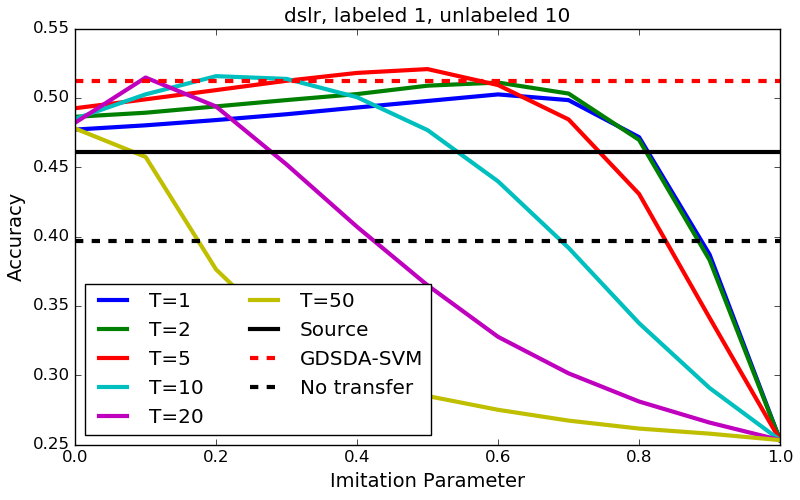
\includegraphics[width=0.2\textwidth]{figure/dslrtoamazonlabeled1unlabeled10.png}}&
\subfloat[15 unlabeled ]{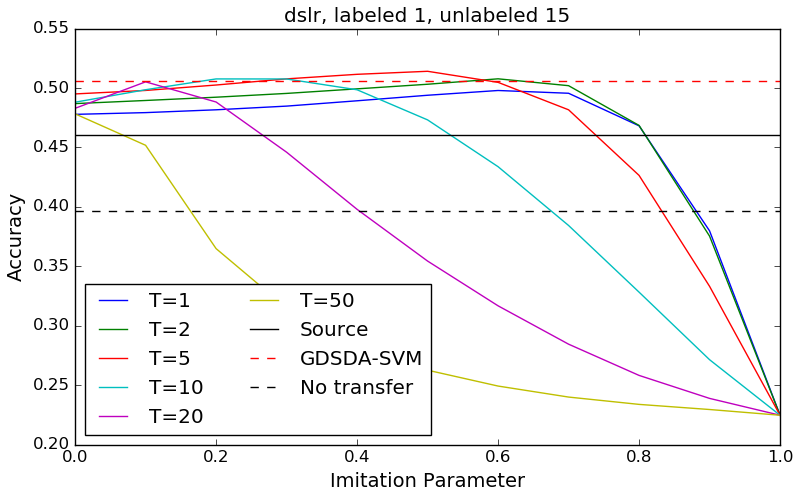
\includegraphics[width=0.2\textwidth]{figure/dslrtoamazonlabeled1unlabeled15.png}}\\
\subfloat[20 unlabeled ]{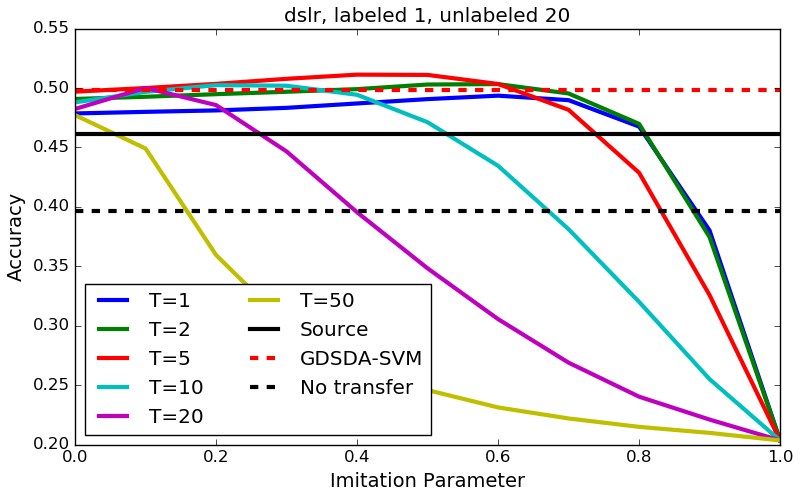
\includegraphics[width=0.2\textwidth]{figure/dslrtoamazonlabeled1unlabeled20.png}}&
\subfloat[10 unlabeled ]{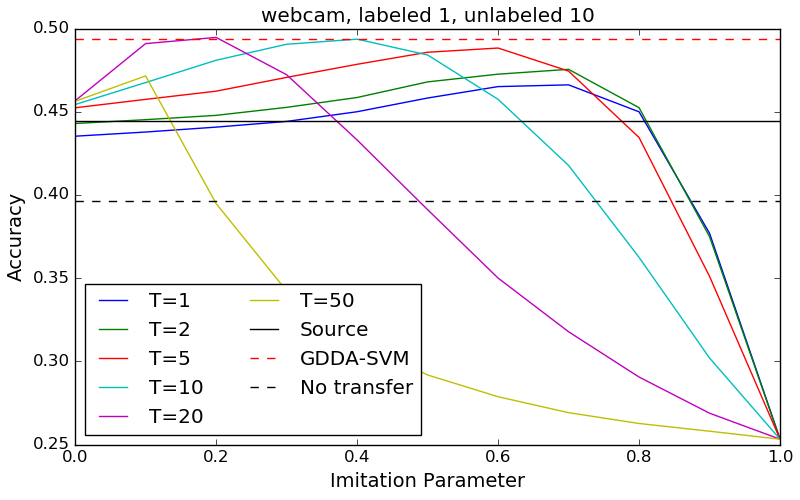
\includegraphics[width=0.2\textwidth]{figure/webcamtoamazonlabeled1unlabeled10.png}}\\
\subfloat[15 unlabeled ]{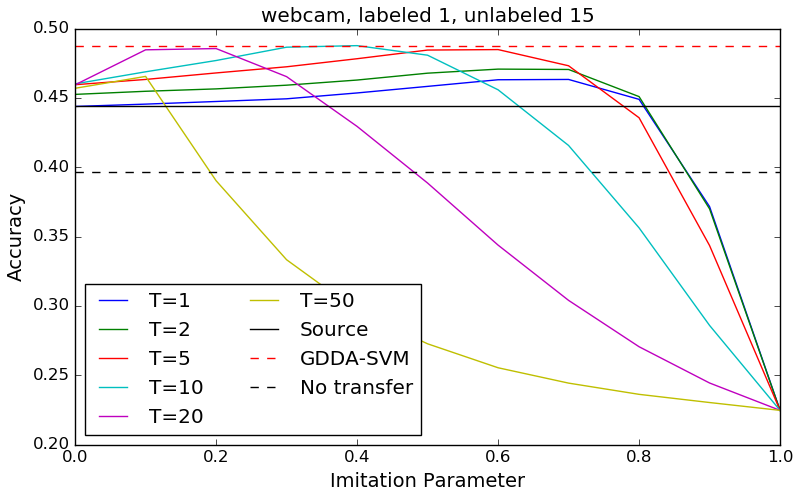
\includegraphics[width=0.2\textwidth]{figure/webcamtoamazonlabeled1unlabeled15.png}}&
\subfloat[20 unlabeled ]{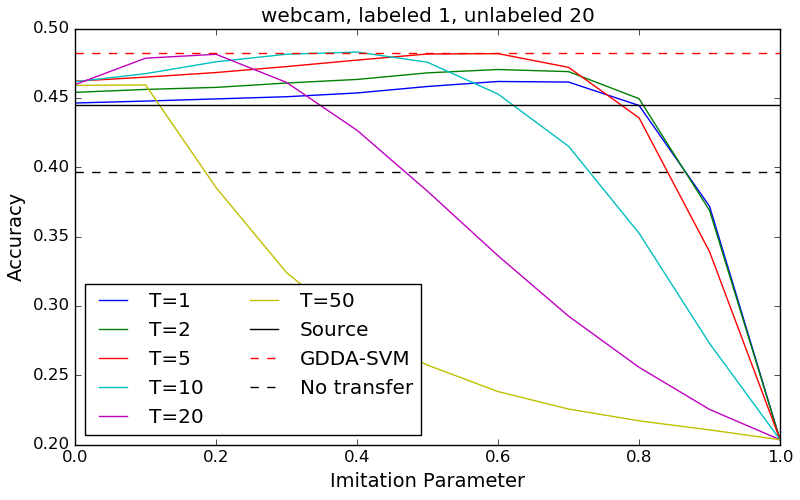
\includegraphics[width=0.2\textwidth]{figure/webcamtoamazonlabeled1unlabeled20.png}}\\
\end{tabular}
\caption{Experiment results on DSLR $\rightarrow$ Amazon and Webcam $\rightarrow$ Amazon when there are just a few labeled examples. The experiments use only 1 labeled example per class. The results of DSLR $\rightarrow$ Amazon and Webcam $\rightarrow$ Amazon are shown in figure (a)-(c) and (d)-(e) respectively. GDDA-SVM is trained with temperature $T=20$.
}\label{fig:single1}
\end{figure}
\subsection{Multi-Source for Office datasets}
In this experiment, the target domain, Amazon dataset, adapts the knowledge from the rest of two source domains, Webcam and DSLR.
We use the identical settings as the single source experiment and perform 2 groups of experiments using 1 labeled and 2 labeled examples per class respectively. We use temperature $T=5$ and the results of multi-source GDDA-SVM is denoted as SVM\_Multi. Here we use two single source GDDA-SVMs (SVM\_w and SVM\_d trained with Webcam and DSLR respectively) as the baselines. We also show the best performance of the brutal force results (SVM\_BF). We search temperature in range $T=[1,2,5,10,20,50]$ and each imitation parameter in range $[0,0.1,...,1]$, making sure that their sum equals 1. The experiment results are shown in Figure \ref{fig:multi}.

From the results, we can see that, when we have 2 source domains, SVM\_Multi can still leverage the knowledge effectively and performs better than any single source model. This shows that the imitation parameter estimated by our method can effectively balance the importance of each source to achieve improved performance. SVM\_Multi performs slightly worse than brutal force result in some experiments. However, considering their time complexity (GDDA-SVM is around 30 times faster than brutal force search), we still think that we still believe that SVM\_Multi is more effectively in real applications.
\begin{figure}
\centering
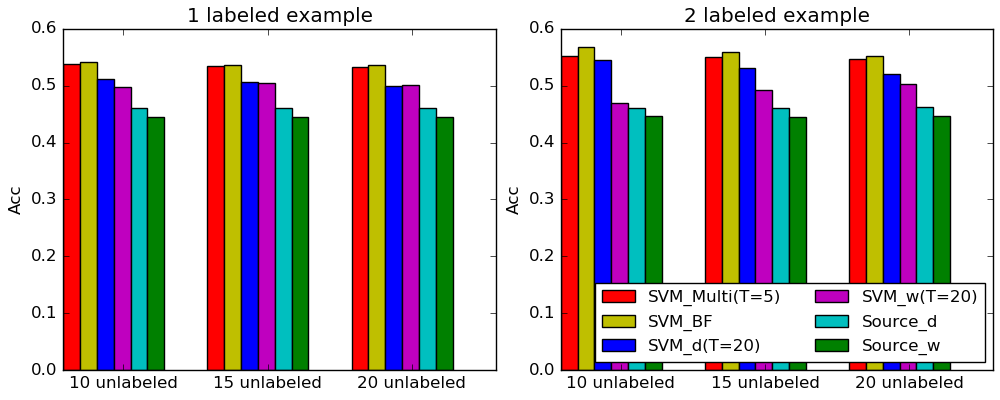
\includegraphics[scale=.3]{figure/cmp.png}
\caption{Multi-source results.}\label{fig:multi}
\end{figure}





\section{Conclusion}\label{sec:con}
In this paper, we propose a framework called \textit{Generalized Distillation Semi-supervised Domain Adaptation} (GDSDA) that can effectively leverage the knowledge from the source domain for SDA problem. We illustrate the effectiveness of GDSDA. In particular, we demonstrate that the knowledge can be effectively transferred between different domains by distillation with the unlabeled examples in the target domain. Moreover, we have shown that the performance of the target model can be further improved with the help of just one labeled example for each class. We also address the importance of the imitation parameter in GDSDA. To make GDSDA more effective in real applications, we proposed a method called GDSDA-SVM which uses SVM as the base learner and can effectively determine the imitation parameter. 
\bibliographystyle{aaai}
\bibliography{research}
\end{document}